%% Net-Gain Scheduling of Parallel Commutators: Rubik's Cubes and Squares up to N = 20
%% acmart, sigconf. `nonacm` drops the ACM rights block for a preprint; remove it (and fill
%% \acmConference, \acmDOI, ...) when targeting a specific ACM venue.
\documentclass[sigconf,nonacm]{acmart}

\usepackage{booktabs}
\usepackage{multirow}
\usepackage[ruled,vlined,linesnumbered]{algorithm2e}
\usepackage{tikz}
\usetikzlibrary{positioning,arrows.meta,fit,calc}
\usepackage{xspace}

\newcommand{\AblCubeCornerMlpPlusTablesNeHTM}{296}
\newcommand{\AblCubeCornerMlpPlusTablesNeSolved}{2/2}
\newcommand{\AblCubeCornerMlpPlusTablesNeTime}{89}
\newcommand{\AblCubeCornerMlpPlusTablesNfHTM}{421}
\newcommand{\AblCubeCornerMlpPlusTablesNfSolved}{2/2}
\newcommand{\AblCubeCornerMlpPlusTablesNfTime}{125}
\newcommand{\AblCubeFullNeHTM}{246}
\newcommand{\AblCubeFullNeSolved}{2/2}
\newcommand{\AblCubeFullNeTime}{31}
\newcommand{\AblCubeFullNfHTM}{452}
\newcommand{\AblCubeFullNfSolved}{2/2}
\newcommand{\AblCubeFullNfTime}{74}
\newcommand{\AblCubeNoCenterMacroRestrictionNeHTM}{246}
\newcommand{\AblCubeNoCenterMacroRestrictionNeSolved}{2/2}
\newcommand{\AblCubeNoCenterMacroRestrictionNeTime}{41}
\newcommand{\AblCubeNoCenterMacroRestrictionNfHTM}{452}
\newcommand{\AblCubeNoCenterMacroRestrictionNfSolved}{2/2}
\newcommand{\AblCubeNoCenterMacroRestrictionNfTime}{133}
\newcommand{\AblCubeNoCoarseTablesNeHTM}{296}
\newcommand{\AblCubeNoCoarseTablesNeSolved}{2/2}
\newcommand{\AblCubeNoCoarseTablesNeTime}{87}
\newcommand{\AblCubeNoCoarseTablesNfHTM}{436}
\newcommand{\AblCubeNoCoarseTablesNfSolved}{2/2}
\newcommand{\AblCubeNoCoarseTablesNfTime}{120}
\newcommand{\AblSquareFullNiHTM}{59}
\newcommand{\AblSquareFullNiSolved}{5/5}
\newcommand{\AblSquareFullNiTime}{0.9}
\newcommand{\AblSquareFullNmHTM}{144}
\newcommand{\AblSquareFullNmSolved}{5/5}
\newcommand{\AblSquareFullNmTime}{4.5}
\newcommand{\AblSquareNoExactStagesNiHTM}{67}
\newcommand{\AblSquareNoExactStagesNiSolved}{5/5}
\newcommand{\AblSquareNoExactStagesNiTime}{0.5}
\newcommand{\AblSquareNoExactStagesNmHTM}{175}
\newcommand{\AblSquareNoExactStagesNmSolved}{5/5}
\newcommand{\AblSquareNoExactStagesNmTime}{4.0}
\newcommand{\AblSquareNoMacrosNiHTM}{59}
\newcommand{\AblSquareNoMacrosNiSolved}{5/5}
\newcommand{\AblSquareNoMacrosNiTime}{15}
\newcommand{\AblSquareNoMacrosNmHTM}{136}
\newcommand{\AblSquareNoMacrosNmSolved}{4/5}
\newcommand{\AblSquareNoMacrosNmTime}{111}
\newcommand{\CuFifteenHTM}{5,280}
\newcommand{\CuFifteenMin}{31}
\newcommand{\CuSolved}{16}
\newcommand{\CuThreeHTM}{52}
\newcommand{\CuTotal}{16}
\newcommand{\CuTwentyHTM}{9,904}
\newcommand{\CuTwentyMin}{79}
\newcommand{\FiveACorrEight}{0.64}
\newcommand{\FiveACorrTen}{0.66}
\newcommand{\FiveACorrTwenty}{0.53}
\newcommand{\FiveACoverage}{$N{=}4$: 10/10, $N{=}5$: 10/10, $N{=}6$: 10/10, $N{=}7$: 4/10, $N{=}8$: 10/10, $N{=}9$: 10/10, $N{=}10$: 8/10, $N{=}12$: 0/1}
\newcommand{\FiveAParams}{198,658}
\newcommand{\FiveASteps}{2,500}
\newcommand{\FiveATrainMin}{35}
\newcommand{\GapFiveAFour}{0.0}
\newcommand{\GapFiveBFour}{7.0}
\newcommand{\GapFiveBThree}{1.2}
\newcommand{\GapMfourFour}{0.0}
\newcommand{\GapMfourThree}{0.0}
\newcommand{\GodSquareFour}{10}
\newcommand{\GodSquareThree}{6}
\newcommand{\MfourEightHTMWFourK}{20.4}
\newcommand{\MfourEightHTMWOneK}{22.0}
\newcommand{\MfourEightHTMWSixteen}{27.3}
\newcommand{\MfourEightHTMWSixtyFour}{38.0}
\newcommand{\MfourEightHTMWTwoFiftySix}{25.3}
\newcommand{\MfourEightSolvedWFourK}{10/10}
\newcommand{\MfourEightSolvedWOneK}{10/10}
\newcommand{\MfourEightSolvedWSixteen}{3/10}
\newcommand{\MfourEightSolvedWSixtyFour}{7/10}
\newcommand{\MfourEightSolvedWTwoFiftySix}{9/10}
\newcommand{\MfourEightTimeWFourK}{17.4}
\newcommand{\MfourEightTimeWOneK}{4.8}
\newcommand{\MfourEightTimeWSixteen}{0.7}
\newcommand{\MfourEightTimeWSixtyFour}{1.4}
\newcommand{\MfourEightTimeWTwoFiftySix}{4.6}
\newcommand{\MfourSolvedWFourK}{60/60}
\newcommand{\MfourSolvedWOneK}{60/60}
\newcommand{\MfourSolvedWSixteen}{52/60}
\newcommand{\MfourSolvedWSixtyFour}{57/60}
\newcommand{\MfourSolvedWTwoFiftySix}{59/60}
\newcommand{\OptFiveAFour}{10/10}
\newcommand{\OptFiveBFour}{0/10}
\newcommand{\OptFiveBThree}{1/10}
\newcommand{\OptMfourFour}{10/10}
\newcommand{\OptMfourThree}{10/10}
\newcommand{\PairedFiveAN}{62}
\newcommand{\PairedFiveAUnseenN}{18}
\newcommand{\PairedMfourN}{60}
\newcommand{\RatioFiveBFiveA}{1.65}
\newcommand{\RatioFiveBFiveAUnseen}{1.20}
\newcommand{\RatioFiveBMfour}{2.35}
\newcommand{\SqNormThree}{0.59}
\newcommand{\SqNormTwenty}{3.64}
\newcommand{\SqSolved}{140}
\newcommand{\SqTotal}{140}
\newcommand{\SqTwentyHTM}{486}
\newcommand{\SqTwentyTime}{60}
\newcommand{\StatesSquareFour}{82,944}
\newcommand{\StatesSquareThree}{768}


\newcommand{\Sq}[1]{#1$\times$#1$\times$1\xspace}
\newcommand{\Cu}[1]{#1$\times$#1$\times$#1\xspace}
\newcommand{\Mfour}{Method~4\xspace}
\newcommand{\FiveA}{Method~5A\xspace}
\newcommand{\FiveB}{Method~5B\xspace}
\newcommand{\FiveC}{Method~5C\xspace}
\newcommand{\Mone}{Method~1\xspace}
\newcommand{\Mtwo}{Method~2\xspace}
\newcommand{\Mthree}{Method~3\xspace}

\begin{document}

\title{Net-Gain Scheduling of Parallel Commutators for Rubik's Cubes and Squares up to $N=20$}
\subtitle{Seven Solvers on One Open Engine, from Exact Search to a Size-Generalizing Network}

%% TODO(authors): add family names, e-mail addresses and the supervising faculty member.
\author{Gaurav}
\affiliation{%
  \institution{Shiv Nadar University}
  \city{Greater Noida}
  \country{India}}
\author{Shree}
\affiliation{%
  \institution{Shiv Nadar University}
  \city{Greater Noida}
  \country{India}}
\author{Sunaina}
\affiliation{%
  \institution{Shiv Nadar University}
  \city{Greater Noida}
  \country{India}}
\author{Kashvi}
\affiliation{%
  \institution{Shiv Nadar University}
  \city{Greater Noida}
  \country{India}}
\author{Shaurya}
\affiliation{%
  \institution{Shiv Nadar University}
  \city{Greater Noida}
  \country{India}}
\author{Sharanya}
\affiliation{%
  \institution{Shiv Nadar University}
  \city{Greater Noida}
  \country{India}}

\renewcommand{\shortauthors}{Gaurav et al.}

\begin{abstract}
Learned Rubik's Cube solvers stop at the \Cu{5} and train a separate network for every size, while
the asymptotically optimal algorithm for large cubes, Demaine et al.'s parallel cluster algorithm, is
rarely implemented and measured against other solvers. We study the \Sq{N} Rubik's Square
and the \Cu{N} Rubik's Cube for every $N$ from 3 to 20 on one open engine, and run seven solvers on
the same seeded instances: IDA* with pattern databases, reduction with Kociemba's two-phase
algorithm, Demaine's parallel algorithm, a CayleyPy-style per-size network, two learned
cluster-based solvers, and a new method. The new method, \FiveC, keeps Demaine's bulk commutators but
schedules them by \emph{net} gain: a bulk move is applied to a whole block of layers when the pieces
it fixes per move beat the best single-cluster fix, even if some cells of the block do not need it.
Every candidate is applied and checked exactly. \FiveC is the shortest method on every cube from
\Cu{5} to \Cu{20} and on the Square from $N=9$ up; on the \Cu{20} it uses \CuTwentyHTMFiveC{} moves,
\FiveCGainTwenty\% fewer than our implementation of Demaine's algorithm and \FiveCvsFiveBTwenty\%
fewer than our staged beam search, and its advantage over Demaine's algorithm grows with $N$
(\FiveCGainSix\% at $N=6$). Exact search gives the ground truth where it can: God's numbers
\GodSquareThree{}, \GodSquareFour{} and \GodSquareFive{} for the \Sq{3}, \Sq{4} and \Sq{5} by
breadth-first search, optimal \Sq{5} solutions by IDA*, and per-size networks that match these optima.
A cluster-token transformer trained only on Squares with $N\le 8$ keeps a correlation of
\FiveACorrTwenty{} with the true scramble depth at $N=20$. All runs are on CPUs; we release the
engine, benchmarks, solvers and every result file.
\end{abstract}

\begin{CCSXML}
<ccs2012>
<concept><concept_id>10010147.10010178.10010205</concept_id>
<concept_desc>Computing methodologies~Search methodologies</concept_desc>
<concept_significance>500</concept_significance></concept>
<concept><concept_id>10010147.10010257</concept_id>
<concept_desc>Computing methodologies~Machine learning</concept_desc>
<concept_significance>300</concept_significance></concept>
<concept><concept_id>10003752.10003809.10003716</concept_id>
<concept_desc>Theory of computation~Mathematical optimization</concept_desc>
<concept_significance>100</concept_significance></concept>
</ccs2012>
\end{CCSXML}
\ccsdesc[500]{Computing methodologies~Search methodologies}
\ccsdesc[300]{Computing methodologies~Machine learning}
\ccsdesc[100]{Theory of computation~Mathematical optimization}

\keywords{Rubik's Cube, heuristic search, parallel algorithms, commutators, beam search,
pattern databases, macro-operators, size generalization, Cayley graphs}

\maketitle

%% =====================================================================
\section{Introduction}

The \Cu{N} Rubik's Cube is a standard testbed for planning on graphs that are far too large to
enumerate. Its worst-case solution length, God's number, is 20 for $N=3$~\cite{rokicki2014diameter}
and grows as $\Theta(N^2/\log N)$~\cite{demaine2011algorithms}; finding a shortest solution of
a given state is NP-complete~\cite{demaine2018npcomplete}. Learned solvers have recently become
strong on small cubes. DeepCubeA~\cite{agostinelli2019deepcubea} and
EfficientCube~\cite{takano2023selfsupervision} solve the \Cu{3}, and the CayleyPy approach of
Chervov et al.~\cite{chervov2025cayleypy} reaches near-optimal \Cu{3} solutions and the first
learned \Cu{4} and \Cu{5} solvers. All of these train one network per size on a one-hot encoding
of the whole sticker array, so a \Cu{6} needs a new model and a new training run, and none
reports a cube beyond $N=5$.

We ask what it takes to cover the whole range $3\le N\le 20$, for both the cube and its flat
relative, the \Sq{N} Rubik's Square of Demaine et al.~\cite{demaine2011algorithms}, and which
approach gives the shortest solutions at each size. The two families share their key structure.
Moves never mix \emph{cubie clusters}, clusters of the same type behave identically at every $N$, and
one slice move touches many clusters at once. Demaine et al.\ use the last fact to solve many
clusters with one shared move sequence; that is what makes $\Theta(N^2/\log N)$ achievable. Our
contributions:

\begin{enumerate}
\item \textbf{An open engine and benchmark} (\S\ref{sec:engine}) for both puzzle families and
  every $N$. Moves come from 3D geometry rather than hand-written tables; clusters are found
  automatically and given a sticker order that does not depend on $N$, so equal cluster types
  have equal \emph{signatures}. A solvability checker, three move metrics and a harness that
  re-applies every returned solution make results comparable across methods.
\item \textbf{A full set of baselines on that engine} (\S\ref{sec:baselines}): IDA* with Korf's
  pattern databases (\Mone), reduction with Kociemba's two-phase algorithm (\Mtwo), Demaine's
  parallel cluster algorithm with 3-cycle batching (\Mthree) and a reproduction of the CayleyPy
  recipe (\Mfour). The commutators that \Mtwo and \Mthree need are found and verified
  automatically for every cluster of every $N$.
\item \textbf{\FiveC, net-gain scheduling of bulk commutators} (\S\ref{sec:5c}), our main new
  method. It keeps Demaine's bulk moves but chooses each one by its net value over a whole block
  of layers, scores every candidate exactly, shares setup moves and looks one step ahead. It is
  the shortest method on every cube from $N=5$ to $N=20$ and on the Square from $N=9$, and its
  lead grows with $N$.
\item \textbf{Two learned cluster-based solvers}: \FiveB (\S\ref{sec:5b}), a staged beam search
  with exact abstraction tables, small cluster networks and machine-verified commutator actions,
  which solved every random state we tested on a two-core CPU; and \FiveA (\S\ref{sec:5a}), a
  cluster-token transformer whose distance estimates carry over to Square sizes it never saw.
\item \textbf{A careful evaluation} (\S\ref{sec:experiments}) on shared, seeded instances,
  including exact God's numbers for the smallest Squares, optimal solutions where IDA* finishes,
  ablations and counting lower bounds. We report where methods fall short, including that exact
  search does not reach random \Cu{3} states on our hardware and that we could not reproduce
  CayleyPy's \Cu{3} result without a GPU.
\end{enumerate}

%% =====================================================================
\section{Related Work}
\label{sec:related}

\paragraph{Structure and complexity.}
Demaine et al.~\cite{demaine2011algorithms} decompose \Sq{N} and \Cu{N} puzzles into cubie
clusters, show that every cluster can be solved without disturbing the others, and obtain
$\Theta(N^2/\log N)$ bounds on the diameter by solving many identical clusters with one shared
move sequence. Optimal solving is NP-complete for both families~\cite{demaine2018npcomplete}.
For the \Cu{3} the diameter is exactly 20 in the half-turn metric~\cite{rokicki2014diameter}.
Their construction batches clusters that are in the \emph{same} configuration; at practical sizes a
cube cluster has about $3\cdot10^{15}$ configurations, so exact matches are rare. \Mthree batches
3-cycles instead, and \FiveC relaxes the batching condition further (\S\ref{sec:5c}).

\paragraph{Classical solvers.}
Korf found optimal \Cu{3} solutions with IDA* and pattern databases~\cite{korf1997optimal},
following Culberson and Schaeffer's pattern databases~\cite{culberson1998pattern}.
Kociemba's two-phase algorithm~\cite{kociemba2phase} and its engineered implementation
min2phase~\cite{chen2phase} give near-optimal \Cu{3} solutions in milliseconds. Large cubes
are usually solved by \emph{reduction} to a \Cu{3}~\cite{walton2017nxnxn}. Korf's
macro-operators~\cite{korf1985macro} learn move sequences that change one part of the state
and restore the rest; our verified commutators play the same role inside a learned search.
The Kaggle Santa 2023 competition~\cite{kaggle2023santa} included large cubes; the KMCoders
write-up~\cite{kmcoders2024santa} reports, for example, a 33$\times$33$\times$33 in 4,719 moves
using cluster-wise 3-cycles applied to many clusters at once, chosen greedily. Their move metric may
differ from ours, so we do not compare lengths directly.

\paragraph{Learned solvers.}
DeepCubeA~\cite{agostinelli2019deepcubea} learns a cost-to-go function by approximate value
iteration and searches with batch weighted A*. EfficientCube~\cite{takano2023selfsupervision}
trains directly on random scrambles from the goal. Q* search~\cite{agostinelli2024qstar}
scores all children of a node in one network pass and handles large action spaces, including
1,872 meta-actions on the \Cu{3}. CayleyPy~\cite{chervov2025cayleypy} trains a residual MLP to
predict the length of a random walk from the solved state (a diffusion distance) and
searches with very wide beams; it reports over 98\% optimal \Cu{3} solutions and the first
learned \Cu{4} and \Cu{5} solvers, and its authors note that the diameter is unknown for every
$N>3$~\cite{chervov2025growth}. All of these models are trained per puzzle size.

\paragraph{Other uses of the cube.}
The cube also serves as a benchmark for robotic manipulation~\cite{openai2019dactyl} and for
spatial reasoning in (multimodal) language models~\cite{anand2025cubebench,gao2025cubebench};
those works use small cubes and do not target solution quality at scale.

\paragraph{Size generalization.}
Networks that read a problem as a set or sequence of parts, such as pointer
networks~\cite{vinyals2015pointer} and set transformers~\cite{lee2019settransformer}, can be
applied to larger instances than they were trained on. \FiveA applies this idea to cubie
clusters.

%% =====================================================================
\section{Problem}
\label{sec:problem}

\paragraph{Puzzles.}
An \Sq{N} Rubik's Square is an $N\times N$ grid of cubies with a top and a bottom colour, plus
side stickers on the border. Its $2N$ moves are 180$^\circ$ flips of one row or one column; each
move is its own inverse. An \Cu{N} Rubik's Cube has $6N^2$ stickers and $3N$ slices; counting a
quarter, half or three-quarter turn of one slice as one move (the half-turn metric, HTM) gives
$9N$ moves. A state is \emph{solved} when every face shows one colour, in any of the reachable
orientations (24 for the cube, 4 for the Square). Given a reachable state, the task is to return
a short move sequence that solves it.

\paragraph{Metrics.}
We report lengths after merging commuting same-axis moves (Section~\ref{sec:engine}) in HTM,
the quarter-turn metric (QTM, where a half turn counts 2) and the slice-turn metric (STM, where a
block of adjacent layers turned together counts 1). For the Square all moves are flips, so
HTM\,=\,QTM. To compare sizes we also divide lengths by $N^2/\ln N$, the growth rate of the
worst case.

\paragraph{Clusters.}
A cubie can only ever reach the positions in its own cluster. Table~\ref{tab:clusters} lists the
cluster types and how many of each an $N$ has; our engine finds them automatically
(\S\ref{sec:engine}) and the counts are checked by unit tests. A \Cu{20} has 2,400 stickers,
9 wing clusters and 81 center clusters; every one must be solved.

\begin{table}[t]
\caption{Cubie cluster types. Wings combine two sticker orbits of one layer. Counts are for one
$N$; $k=\lfloor N/2\rfloor-1$.}
\label{tab:clusters}
\small
\begin{tabular}{@{}llrl@{}}
\toprule
Puzzle & Cluster type & Stickers & Count \\
\midrule
Cube & corners & 24 & 1 \\
     & middle edges & 24 & 1 if $N$ odd \\
     & wing edges & 48 & $k$ \\
     & centers ($+$, $\times$, oblique) & 24 & $((N-2)^2-[N\text{ odd}])/4$ \\
     & fixed centers & 6 & 1 if $N$ odd \\
\midrule
Square & corner & 16 & 1 \\
       & edge & 12 & $2k$ \\
       & interior & 8 & $k^2$ \\
       & edge-cross, cross, center & 6, 4, 2 & odd $N$ only \\
\bottomrule
\end{tabular}
\end{table}

%% =====================================================================
\section{Engine and Benchmark}
\label{sec:engine}

All methods run on one engine~\cite{rubikrepo}. Everything below is generic over cuboid
dimensions $(d_0,d_1,d_2)$, so the cube $(N,N,N)$ and the Square $(N,N,1)$ come from the same code.

\paragraph{Moves from geometry.}
Each sticker stores a doubled, centred cubie coordinate and an outward normal. A move rotates
every sticker of one slab by an integer rotation matrix; looking up the rotated
(position, normal) pair gives a permutation $\pi$, and applying the move is the gather
$s\leftarrow s[\pi]$. A slab whose cross-section is not square, such as one row of the Square,
only gets 180$^\circ$ turns, and an axis of length 1 gets none. Unit tests check that every move
has order 4 (or 2) and that each move followed by its inverse is the identity, for every tested
$N$.

\paragraph{Canonical form.}
Moves on the same axis commute. We canonicalise a sequence by merging each same-axis run per
layer and sorting by layer, and we use the same order to prune search: after a move on axis
$a$, layer $\ell$, no move on axis $a$ with layer $\le\ell$ is allowed. This removes immediate
repeats and every redundant ordering of commuting moves.

\paragraph{Clusters with $N$-invariant signatures.}
Union-find over all move permutations gives the sticker orbits; orbits sharing cubies are merged
into cubie clusters. Inside a cluster, stickers are sorted by face and by the signs and relative
magnitudes of their in-face coordinates. This order does not depend on $N$, so the moves acting
on a cluster induce the same local permutations at every $N$. We hash the local generator set
and the solved pattern into a \emph{signature}; tests confirm that, for example, every
$\times$-center cluster of the \Cu{5}, \Cu{7} and \Cu{9} has the same signature. A model trained
for one cluster type therefore applies at any size.

\paragraph{Projections.}
Restricting attention to a subset of stickers gives a \emph{projected puzzle}. When it is small
we enumerate it by breadth-first search from the solved pattern; the resulting table gives exact
distances for that subset and doubles as an exact membership test.

\paragraph{Solvability checker.}
A state is accepted only if it passes: global and per-cluster colour counts; membership in the
exact projection table for every cluster small enough to enumerate (all Square clusters); for
cubes, valid corner, middle-edge and wing pieces, corner twist $\equiv 0 \pmod 3$ and, for odd
$N$ after normalising orientation by the fixed centers, even middle-edge flip and equal corner
and middle-edge permutation parity; and for the Square, joint consistency of each cross cluster
with the border clusters it shares moves with. These are necessary conditions. Property tests
confirm that the checker accepts scrambled states and rejects a single corner twist, a single
middle-edge flip, a swap of two corners on odd cubes and wrong colour counts.

\paragraph{Harness.}
Every solver implements one interface and returns engine moves. The harness re-applies the
moves, decides \emph{solved} itself, and writes one row per instance with lengths in all three
metrics, time, nodes, memory, seed, hardware and git commit. A crash or time-out counts as a
failure and stays in the denominator.

\paragraph{Shared beam search.}
Methods 4, 5A and 5B share one beam search. Per step it expands the beam in chunks, scores
children with the heuristic, and keeps the $W$ best after removing duplicates by a random
64-bit linear hash (also across the last three steps). Only (score, hash, parent, action) is
stored per child; the next beam is rebuilt from parents. Beam states are packed at 3 bits per
sticker and can live on the device, in pinned host memory or on disk. The search accepts
\emph{macro actions}: fixed move sequences applied as one step and expanded into ordinary moves in
the output. A heuristic that can score all children of a parent in one pass is used that way,
as in Q* search~\cite{agostinelli2024qstar}.

\paragraph{Instances.}
Random states are long random canonical walks (at least $25\times$ the number of moves, and at
least 400 moves). This approximates, but does not guarantee, a uniform random reachable state.
Every instance is regenerated from a seed and checked by the solvability checker; all methods
see the same instances.

%% =====================================================================
\section{Baselines: Methods 1--4}
\label{sec:baselines}

\paragraph{Pure 3-cycles for any cluster.}
\Mtwo and \Mthree need, for every center and wing cluster of every $N$, move sequences that
3-cycle three of its pieces and touch nothing else. We find them automatically. For centers we
enumerate commutators $[A, B\,C\,B']$ with $A$ and $C$ inner-slice quarter turns on one axis and
$B$ an outer face turn; for wings, $[X, Y\,Z\,Y']$ with $X$ an inner slice and $Y, Z$ outer faces.
A candidate is kept if, applied to the sticker permutation, it moves exactly three cubies of one
cluster. A conjugate $s\,c\,s'$ of a pure 3-cycle $c$ is again pure, so breadth-first search over
setup moves $s$ (up to four) extends a few base commutators to every one of the
$24\cdot23\cdot22/3$ 3-cycles of a cluster, each with a short move sequence. A greedy solver then
applies, at each step, the 3-cycle with the most pieces fixed per move.

\paragraph{\Mone: IDA* with pattern databases.}
For the \Cu{3} we use Korf's heuristic~\cite{korf1997optimal}: the maximum of a corner database
($8!\cdot3^7 = 88{,}179{,}840$ entries) and two 6-edge databases ($12!/6!\cdot2^6 = 42{,}577{,}920$
each), built by breadth-first search over cubie coordinates whose move tables are derived from the
engine's sticker permutations (a test checks they agree). IDA* runs in Numba, parallel over the
root's moves, at about $1.2\cdot10^7$ nodes per second on four cores, with the canonical move order
of \S\ref{sec:engine}. For the Square the heuristic is the maximum over clusters of each cluster's
exact distance, which is admissible because no solution fixes a cluster in fewer moves than it needs
alone; since any of the four solved orientations counts, IDA* runs to each of them and keeps the
shortest. For the smallest Squares, breadth-first search from all four solved orientations gives the
exact distance of every state.

\paragraph{\Mtwo: reduction with Kociemba's two-phase algorithm.}
After relabelling colours so that the target is one fixed orientation (for odd $N$ the fixed
centers decide), the cube is solved in four stages, each a function from state to moves:
(i) every wing cluster with an odd permutation gets one inner-slice quarter turn (Demaine's
Lemma~7); (ii) every center cluster is solved with its pure 3-cycles; (iii) corners, middle edges
and fixed centers, which behave as a \Cu{3} under outer-face turns, are solved by Kociemba's
two-phase algorithm~\cite{kociemba2phase}; for even $N$ an odd corner permutation (PLL parity) is
fixed by one outer quarter turn first; (iv) every wing cluster is solved with its pure 3-cycles.
Outer-face turns keep center clusters on their faces, and pure 3-cycles keep everything else, so the
stages never undo each other. On the Square, \Mtwo solves the frame and the edge and cross clusters
exactly on their projections (Demaine's Lemma~3, $O(N)$ moves) and then each interior cluster with
its four commutators $c\,r\,c\,r$ (Lemma~2), at most three each.

\paragraph{\Mthree: Demaine's parallel algorithm.}
\Mthree shares every stage with \Mtwo except the batching. On the Square, each interior cluster's
optimal word of commutators is read off its exact table; round $t$ applies the $t$-th commutator of
every cluster, and the clusters needing the same commutator are covered by blocks of columns $X$ and
rows $Y$, each fixed by one bulk sequence $C_X R_Y C_X R_Y$ of $2|X|+2|Y|$ moves (Lemma~4), with
Demaine's column groups (Lemmas~5--6). On the cube, batching by identical configuration is useless at
practical sizes, so, as the KMCoders write-up suggests~\cite{kmcoders2024santa}, we batch 3-cycles.
A commutator \emph{type} is an outer-face setup plus a template with layer parameters, such as
$[A_i, B\,C_j\,B']$; with layer sets $I$ and $J$ (all slices of $I$ turned together) it applies the same
3-cycle pattern to every cluster $(i,j)\in I\times J$ for $2|I|+2|J|+4$ moves. Each round picks the type
with the most pieces fixed per move over all clusters, applies it to every block of clusters that it
helps, or applies one single-cluster 3-cycle when that is better.

\paragraph{\Mfour: CayleyPy reproduction.}
\Mfour re-implements the recipe of Chervov et al.~\cite{chervov2025cayleypy} on our engine: one
residual MLP per puzzle size on one-hot sticker inputs, trained with MSE on fresh non-backtracking
random walks to predict walk length, and beam search with hash deduplication for at most 200
steps. Square models have 0.25--0.45M parameters and were trained on 4M (N $\le$ 5) or 10M
(N = 6--8) examples in 1--4 minutes each on CPU. We also trained the paper's 4.0M-parameter
\Cu{3} model on 32M examples (77 minutes on CPU), 250$\times$ fewer than the paper's 8B.

%% =====================================================================
\section{Method 5C: Net-Gain Scheduling of Bulk Commutators}
\label{sec:5c}

\Mthree applies a commutator type to a block $X\times Y$ of layer pairs only when \emph{every} cell
of the block helps the cluster it acts on. Early on many clusters need the same 3-cycle and blocks
are large, but the clusters soon diverge, the blocks shrink to single cells and batching fades:
on our \Cu{20}, \MthreeSingleRoundsTwenty{} of \Mthree's \MthreeRoundsTwenty{} center rounds fixed
a single cluster. \FiveC changes only this schedule.

\paragraph{Net-gain blocks.}
For a type $t$, let $g_t(i,j)$ be the change in the number of solved pieces of the cluster that cell
$(i,j)$ acts on; it can be zero or negative. Let $\lambda$ be the best number of pieces per move that
any single-cluster 3-cycle offers in the current state. \FiveC chooses
\begin{equation}
(X^\ast,Y^\ast)=\arg\max_{X\cap Y=\emptyset}\;\sum_{(i,j)\in X\times Y} g_t(i,j)\;-\;\lambda\,\bigl(2|X|+2|Y|+4+2|s_t|\bigr),
\end{equation}
where $s_t$ is the type's setup and every cell of $X\times Y$ must be a verified pure 3-cycle. A block is
worth applying exactly when its pieces per move beat the best single fix, so cells that do not help,
or slightly hurt, are accepted when the block still pays. We maximise by alternation (rows given
columns, columns given rows) from the three best rows. Because several cells may act on one cluster,
each candidate is then \emph{applied} to the state and scored exactly; this also checks that nothing
outside the clusters moved. Wings have one layer parameter and the same rule with $Y$ omitted.

\paragraph{Setup sharing and lookahead.}
A type whose setup equals the previous step's is charged $2|s_t|$ moves less, because the shared
$s_t'\,s_t$ cancels when moves are canonicalised. With one step of lookahead (used for $N\le15$, where
it is affordable), the four best candidates are re-scored by the best step available after them.

\paragraph{Everything else is \Mthree.}
Wing parity, the \Cu{3} stage, the Square frame and edge stages, the type bank and the single-cluster
fallback are shared with \Mthree, so the difference between the two methods is the schedule alone. On
the Square, the net-gain schedule of the interior clusters (gain = drop in exact distance) and \Mthree's
are both computed, in milliseconds, and the shorter is kept.

\begin{algorithm}[t]
\caption{\FiveC schedule for one family of clusters (centers or wings)}
\label{alg:5c}
\small
\KwIn{state $s$; type bank (verified pure 3-cycles per type, cluster and layers); per-cluster 3-cycle libraries}
\KwOut{move sequence $\mu$ solving every cluster of the family}
$\mu\leftarrow[\,]$\;
\While{some cluster is unsolved}{
  $c_1\leftarrow$ best single-cluster 3-cycle; $\lambda\leftarrow$ pieces fixed per move of $c_1$\;
  \For{each of the 24 types with the largest total positive gain}{
    $(X,Y)\leftarrow$ alternating maximisation of Eq.~2\;
    apply the bulk commutator to $s$; discard it if anything outside the clusters moved\;
    record its exact gain and its moves (less shared setup)\;}
  pick the best gain per move among the blocks and $c_1$ (optionally after one step of lookahead)\;
  $s\leftarrow s\cdot\nu$;\quad $\mu\leftarrow\mu\,\Vert\,\nu$\;
}
\Return $\mu$\;
\end{algorithm}

%% =====================================================================
\section{Method 5B: Cluster-Decomposed Staged Beam Search}
\label{sec:5b}

\FiveB solves the puzzle in a sequence of stages (Figure~\ref{fig:pipeline},
Algorithm~\ref{alg:5b}). Each stage adds a few pieces to an exact goal: those pieces, and every
piece solved by an earlier stage, must show their solved stickers. Each stage is a small search
problem with a sharp signal, and later stages cannot silently undo earlier work.

\begin{figure}[t]
\centering
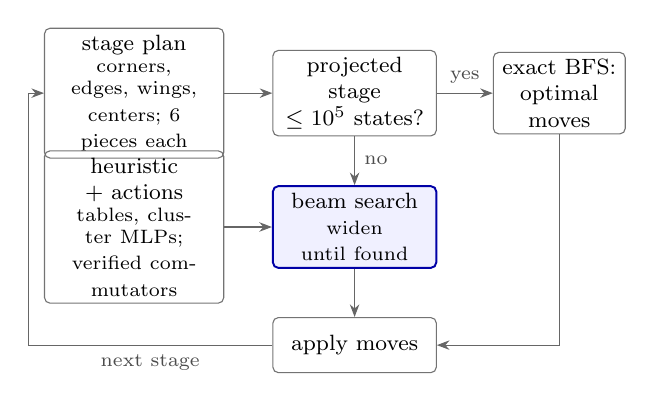
\begin{tikzpicture}[font=\footnotesize,
  box/.style={draw=black!55, rounded corners=2pt, align=center, inner sep=2.5pt, minimum height=7mm},
  hl/.style={box, draw=blue!65!black, fill=blue!6, line width=0.7pt},
  ar/.style={-{Stealth[length=1.6mm]}, draw=black!60}, lab/.style={font=\scriptsize, text=black!70}]
\node[box, text width=21mm] (plan) at (0,0) {stage plan\\{\scriptsize corners, edges, wings,\\centers; 6 pieces each}};
\node[box, text width=19mm] (small) at (28mm,0) {projected stage\\$\le 10^5$ states?};
\node[box, text width=15mm] (bfs) at (54mm,0) {exact BFS:\\optimal moves};
\node[box, text width=21mm] (inp) at (0,-17mm) {heuristic + actions\\{\scriptsize tables, cluster MLPs;\\verified commutators}};
\node[hl, text width=19mm] (beam) at (28mm,-17mm) {beam search\\{\scriptsize widen until found}};
\node[box, text width=19mm] (apply) at (28mm,-32mm) {apply moves};
\draw[ar] (plan) -- (small);
\draw[ar] (small) -- node[lab, above]{yes} (bfs);
\draw[ar] (small) -- node[lab, right]{no} (beam);
\draw[ar] (inp) -- (beam);
\draw[ar] (beam) -- (apply);
\draw[ar] (bfs.south) |- (apply.east);
\draw[ar] (apply.west) -- node[lab, below]{next stage} ++(-31mm,0) |- (plan.west);
\end{tikzpicture}
\caption{\FiveB. Each stage adds a few pieces to an exact goal. Tiny stages are solved
optimally by lookup; the rest by beam search over single moves and verified commutators, guided
by exact abstraction tables and small cluster networks.}
\label{fig:pipeline}
\end{figure}

\paragraph{Stage plan.}
For the Square we follow Demaine et al.~\cite{demaine2011algorithms}: the \emph{frame} (corner,
center and edge-cross clusters), then edge clusters two at a time, then cross clusters and interior
clusters three at a time, from the outside in. For the cube we use an \emph{edges-first} order:
fixed centers, corners, middle edges, wings, then centers, with every wing and center cluster split
into stages of 6 pieces. Inner-slice moves never disturb corners, and the commutators below never
disturb edges, so the later and more numerous stages have cheap actions that keep earlier work.

\paragraph{Stage actions.}
A move that touches none of the current targets cannot make progress, so each stage searches
only the single moves that touch a target plus the macro actions that do. This cuts the
branching factor from $O(N^2)$ macros to a handful. The macro pool is:
\begin{itemize}
\item \emph{Square}: for every row $r$ and column $c$, the commutator $c\,r\,c\,r$, which changes
  only the cluster at their crossing (Demaine's Lemma~2), and the conjugates $r\,c\,r$ and
  $c\,r\,c$; $3N^2$ macros.
\item \emph{Cube}: $X\,Y\,X'\,Y'$ for an inner-slice quarter turn $X$ and an outer-face quarter
  turn $Y$ on another axis, which never moves corners; and pure-center commutators
  $[A, B\,C\,B'] = A\,B\,C\,B'\,A'\,B\,C'\,B'$ with $A$ and $C$ inner-slice quarter turns on one axis
  (the middle slice included, e.g.\ $[M, U\,r\,U']$) and $B$ a face turn on another axis.
  Every candidate is applied to the sticker permutation and kept only if it moves center stickers
  alone; duplicates with the same permutation are dropped. This leaves 192 pure-center
  commutators for the \Cu{4} and 29,376 for the \Cu{20}, and covers all 81 center clusters
  of the \Cu{20}.
\end{itemize}
Once every corner and edge is solved, a center stage searches \emph{only} the pure-center
commutators, which keep all earlier work by construction.

\paragraph{Heuristics.}
A stage's heuristic is a weighted sum over clusters:
\begin{equation}
h(s)=\sum_{c\in T} h_c(s) + \lambda_{\text{keep}}\!\!\sum_{c\in P} h_c(s)
     + \lambda_{\text{ex}}\,\bigl|\{i\in G: s_i\ne s^\ast_i\}\bigr| ,
\end{equation}
where $T$ are the target clusters, $P$ the earlier clusters that some allowed action can move,
$G$ the stage's goal stickers and $s^\ast$ the solved state ($\lambda_{\text{keep}}=1$,
$\lambda_{\text{ex}}=0.5$). Each per-cluster term $h_c$, shared by signature across all $N$, is
one of three kinds:
\begin{enumerate}
\item \emph{Exact table}, when the projected cluster has at most 1.5M states: every Square
  cluster and the fixed centers.
\item \emph{Coarse abstraction tables}: the projection after mapping one pair of opposite
  colours to 1 and the rest to 0. These are pattern databases over a colour
  abstraction~\cite{culberson1998pattern} and give admissible lower bounds. They have
  2,187 states for corners, 126,720 for middle edges and 735,471 for every center type; wings
  are skipped because every such projection exceeds the cap. For corners a finer three-class
  abstraction (one colour to 1, its opposite to 2) has 153,090 states.
\item \emph{Cluster MLP}: a small residual MLP (hidden width 256, two residual blocks) trained on
  random walks of the projected cluster to predict walk length, combined with the coarse tables
  by $\max$. Six such networks (corner, middle edge, wing, three center types) cover every
  cube size; each trained for 1,500 steps on CPU in 2--15 minutes.
\end{enumerate}
Corners use the three-class tables alone. The MLP's walk-length targets overestimate the true
distance, and taking the max with them flattens the tables' signal; Section~\ref{sec:ablations}
measures the effect.

\paragraph{Exact small stages.}
If the projection of a stage's goal stickers under the stage's single moves has at most 100,000
states, we enumerate it and descend greedily on the exact distances, which is optimal for that
stage. The Square frame always qualifies: for any $N$ it depends only on rows and columns $0$,
$\lfloor N/2\rfloor$ and $N-1$, and is therefore a \Sq{3} with at most 768 states.

\paragraph{Width schedule.}
Each stage starts at width $W_0$ (128 for the Square, 512 for the cube) and, if it fails within its
step limit (40 and 60 steps), retries at $4\times$ the width up to $W_{\max}$ (2,048 and 8,192).
Stages with few actions may widen further while $W\times|\text{actions}|\le 1.2\cdot 10^6$; the
18-action \Cu{3} corner stage thus reaches $2^{16}$.

\begin{algorithm}[t]
\caption{\FiveB (one state)}
\label{alg:5b}
\small
\KwIn{state $s$, stage plan $S_1,\dots,S_m$}
\KwOut{move sequence $\mu$ with $s\cdot\mu$ solved}
$\mu\leftarrow[\,]$\;
\For{$i\leftarrow1$ \KwTo $m$}{
  $G\leftarrow\bigcup_{j\le i}\text{goal}(S_j)$\;
  \lIf{$s$ already solved on $G$}{\textbf{continue}}
  $A\leftarrow$ single moves and verified macros that move some target of $S_i$\;
  \uIf{projection of $G$ under $A$ has $\le 10^5$ states}{
    $\nu\leftarrow$ optimal moves by greedy descent on its BFS table\;}
  \Else{
    $h\leftarrow$ stage heuristic (Eq.~1)\;
    $W\leftarrow W_0$\;
    \Repeat{$\nu$ found \textbf{or} $W > W_{\max}(|A|)$}{
      $\nu\leftarrow$ \textsc{BeamSearch}$(s, A, h, W, \text{goal}=G)$\;
      $W\leftarrow4W$\;}
  }
  \lIf{no $\nu$}{\Return failure}
  $s\leftarrow s\cdot\nu$;\quad $\mu\leftarrow\mu\,\Vert\,\nu$\;
}
\Return canonicalise$(\mu)$\;
\end{algorithm}

%% =====================================================================
\section{Method 5A: One Network for Every Size}
\label{sec:5a}

\FiveA replaces the per-size sticker network with one that reads the puzzle as a set of cluster
tokens. Each cluster becomes one token: the one-hot colours of its stickers in the canonical order,
projected by a linear map shared by all clusters of the same type, plus a learned embedding of the
cluster kind and a small MLP of geometric features (the cluster's two in-face depths divided by
$N-1$, and $N/20$). A transformer encoder~\cite{vaswani2017attention} without positional order
mixes the tokens, since they form a set~\cite{lee2019settransformer}. The value head is
\emph{additive}: each token predicts a non-negative cost, the costs are summed, and a small global
correction is added. A sum matches the structure of the problem, since total distance grows with the
number of unsolved clusters, and it extends to any number of tokens. The per-token costs also serve as
per-cluster heuristics inside \FiveB's stages.

Training uses fresh non-backtracking random walks from the solved state on every training size,
with the walk length $k$ as target and the loss on $(\hat k-k)/(N^2/\ln N)$ so that all sizes
contribute on one scale. The model we evaluate has \FiveAParams{} parameters (width 64, two layers,
four heads) and was trained for \FiveASteps{} steps on Squares with $N\in\{4,\dots,8\}$ only, in
\FiveATrainMin{} minutes on CPU. At test time it runs full-puzzle beam search for $N\le7$ and,
above that, \FiveB's stages with its per-token costs as the stage heuristic. The architecture
also has a Q*-style move head; we did not evaluate it.

%% =====================================================================
\section{Experiments}
\label{sec:experiments}

\paragraph{Setup.}
All runs used CPUs without a GPU. \FiveB, \FiveA and \Mfour ran on a 2-core machine with one thread per
process; Methods 1--3 and \FiveC ran on a 4-core machine, one process per run (\Mone's \Cu{3} search
uses all four cores). Square experiments use 10 seeded random states for $N\le12$ and 5 for
$13\le N\le20$; cube experiments use 2 states for $N\le10$ and one each for $N=15$ and $N=20$. Every
method sees the same instances, and every number below comes from the harness's result files, from
which our tables and figures are generated by script. Means are over solved instances; a superscript
gives the solved fraction when it is below 100\%. Times are comparable within a machine only.

%% Results section. Every table body is generated by paper/scripts/make_tables.py.

\subsection{Coverage: every size, both puzzles}
\label{sec:coverage}

\begin{table*}[t]
\caption{Rubik's Square, random states. Columns: number of instances; mean optimal length (exact
BFS, $N\le4$); mean HTM of \Mfour (per-size network, $W{=}4096$), \FiveA and \FiveB on the same
instances; \FiveB's solved fraction, its length divided by $N^2/\ln N$, and its mean time per
state. A superscript gives the solved fraction when below 100\%; ``--'' = not run (no model for that
size), and ``--$^{0/k}$'' = tried, none solved.}
\label{tab:square}
\small
\begin{tabular}{@{}rrrrrrrrr@{}}
\toprule
$N$ & $n$ & optimal & \Mfour & \FiveA & \FiveB HTM\,$\pm$\,95\% CI & \FiveB solved & \FiveB / $(N^2/\ln N)$ & \FiveB time (s) \\
\midrule
3 & 10 & 3.6 & 3.6 & -- & 4.8\,$\pm$\,1.0 & 10/10 & 0.59 & 0.0 \\
4 & 10 & 6.4 & 6.4 & 6.4 & 13.4\,$\pm$\,1.8 & 10/10 & 1.16 & 0.0 \\
5 & 10 & -- & 8.8 & 10.0 & 22.2\,$\pm$\,2.3 & 10/10 & 1.43 & 0.2 \\
6 & 10 & -- & 13.0 & 15.0 & 28.0\,$\pm$\,2.5 & 10/10 & 1.39 & 0.1 \\
7 & 10 & -- & 15.0 & 23.5$^{4/10}$ & 41.8\,$\pm$\,4.4 & 10/10 & 1.66 & 0.2 \\
8 & 10 & -- & 20.4 & 56.4 & 61.6\,$\pm$\,5.4 & 10/10 & 2.00 & 0.6 \\
9 & 10 & -- & -- & 70.0 & 83.2\,$\pm$\,6.1 & 10/10 & 2.26 & 1.0 \\
10 & 10 & -- & -- & 85.5$^{8/10}$ & 103.4\,$\pm$\,6.1 & 10/10 & 2.38 & 1.6 \\
11 & 10 & -- & -- & -- & 121.4\,$\pm$\,7.5 & 10/10 & 2.41 & 3.3 \\
12 & 10 & -- & -- & --$^{0/1}$ & 143.0\,$\pm$\,6.4 & 10/10 & 2.47 & 5.9 \\
13 & 5 & -- & -- & -- & 170.4\,$\pm$\,7.3 & 5/5 & 2.59 & 7.0 \\
14 & 5 & -- & -- & -- & 221.2\,$\pm$\,17.6 & 5/5 & 2.98 & 11.9 \\
15 & 5 & -- & -- & -- & 242.8\,$\pm$\,20.9 & 5/5 & 2.92 & 13.0 \\
16 & 5 & -- & -- & -- & 280.0\,$\pm$\,15.8 & 5/5 & 3.03 & 15.8 \\
17 & 5 & -- & -- & -- & 298.4\,$\pm$\,30.8 & 5/5 & 2.93 & 21.1 \\
18 & 5 & -- & -- & -- & 354.8\,$\pm$\,11.5 & 5/5 & 3.17 & 34.0 \\
19 & 5 & -- & -- & -- & 394.4\,$\pm$\,23.5 & 5/5 & 3.22 & 43.0 \\
20 & 5 & -- & -- & -- & 486.4\,$\pm$\,43.3 & 5/5 & 3.64 & 60.3 \\
\bottomrule

\end{tabular}
\end{table*}

\begin{table}[t]
\caption{Rubik's Cube, random states, \FiveB. Time is wall-clock seconds per state.}
\label{tab:cube}
\small\setlength{\tabcolsep}{4pt}
\begin{tabular}{@{}rrrrrrr@{}}
\toprule
$N$ & $n$ & solved & HTM & QTM & HTM/$(N^2/\ln N)$ & time (s) \\
\midrule
3 & 2 & 52.0 & \textbf{21.0} & \textbf{21.0} & \textbf{21.0} & 31.0 & 2.6 & 0 \\
4 & 2 & 246.0 & 219.0 & \textbf{192.5} & 196.0 & 224.5 & 17.0 & 1 \\
5 & 2 & 452.5 & 319.5 & 258.0 & \textbf{253.0} & 281.0 & 16.3 & 1 \\
6 & 2 & 724.5 & 574.5 & 464.5 & \textbf{437.0} & 481.5 & 21.7 & 4 \\
7 & 2 & 1,045.0 & 811.0 & 633.0 & \textbf{564.0} & 614.5 & 22.4 & 7 \\
8 & 2 & 1,510.5 & 1,131.0 & 897.5 & \textbf{806.5} & 863.0 & 26.2 & 17 \\
10 & 2 & 2,260.5 & 1,900.5 & 1,509.0 & \textbf{1,196.5} & 1,256.5 & 27.6 & 37 \\
15 & 1 & 5,280.0 & 4,565.0 & 3,578.0 & \textbf{2,765.0} & 2,927.0 & 33.3 & 223 \\
20 & 1 & 9,904.0 & 8,259.0 & 6,612.0 & \textbf{4,925.0} & 5,188.0 & 36.9 & 158 \\
\bottomrule

\end{tabular}
\end{table}

\FiveB solved all \SqSolved{} of \SqTotal{} Square instances (Table~\ref{tab:square}) and all
\CuSolved{} of \CuTotal{} cube instances (Table~\ref{tab:cube}). The \Sq{20} took
\SqTwentyTime{}\,s per state on average; the \Cu{15} took \CuFifteenMin{} minutes
(\CuFifteenHTM{} moves) and the \Cu{20} \CuTwentyMin{} minutes (\CuTwentyHTM{} moves). To our
knowledge no earlier learned-search solver has been reported beyond the
\Cu{5}~\cite{chervov2025cayleypy}. The price is length: \FiveB's \Cu{3} solutions average
\CuThreeHTM{} HTM, against an optimum of about 18 on random states~\cite{rokicki2014diameter}.

\subsection{Distance from optimal on small Squares}
\label{sec:optimal}

The \Sq{3} and \Sq{4} are small enough to enumerate. Breadth-first search from all four solved
orientations visits \StatesSquareThree{} and \StatesSquareFour{} states; their diameters are
\GodSquareThree{} and \GodSquareFour{} moves. Table~\ref{tab:optimal} scores each method against
the exact optimum on the same instances. The per-size network of \Mfour found the optimum on every
instance (\OptMfourThree{} and \OptMfourFour{}). \FiveB was \GapFiveBThree{} and \GapFiveBFour{}
moves above it on average: its stages fix pieces in a prescribed order and pay for commutators
that a global search does not need.

\begin{table}[t]
\caption{Optimality on the smallest Squares. ``Gap'' = mean HTM above the exact optimum over
solved instances; ``optimal'' = instances solved in exactly the optimal length. \FiveA was
evaluated for $N\ge4$ only.}
\label{tab:optimal}
\small\setlength{\tabcolsep}{4pt}
\begin{tabular}{@{}lrrlrrr@{}}
\toprule
Puzzle & God's & mean opt. & Method & solved & gap & optimal \\
\midrule
\multirow{3}{*}{3$\times$3} & \multirow{3}{*}{6} & \multirow{3}{*}{3.6} & Method 4 ($W{=}4096$) & 10/10 & 0.0 & 10/10 \\
 & &  & Method 5A & -- & -- & -- \\
 & &  & Method 5B & 10/10 & 1.2 & 1/10 \\
\midrule
\multirow{3}{*}{4$\times$4} & \multirow{3}{*}{10} & \multirow{3}{*}{6.4} & Method 4 ($W{=}4096$) & 10/10 & 0.0 & 10/10 \\
 & &  & Method 5A & 10/10 & 0.0 & 10/10 \\
 & &  & Method 5B & 10/10 & 7.0 & 0/10 \\
\bottomrule

\end{tabular}
\end{table}

\subsection{Comparison with per-size networks}
\label{sec:pernetwork}

\Mfour's per-size networks are the strongest method we have on the sizes where they exist.
On the \PairedMfourN{} Square instances with $3\le N\le8$ that both methods solved, \FiveB's
solutions were on average \RatioFiveBMfour$\times$ as long as \Mfour's at $W{=}4096$
(Table~\ref{tab:square}). As CayleyPy reports for cubes~\cite{chervov2025cayleypy}, wider beams
help (Figure~\ref{fig:m4width}). They also decide coverage at the largest trained size: on the
\Sq{8}, \Mfour solved \MfourEightSolvedWSixteen{} states at $W{=}16$,
\MfourEightSolvedWTwoFiftySix{} at $W{=}256$ and all from $W{=}1024$ on, at
\MfourEightTimeWFourK\,s per state for $W{=}4096$. The cost is a separate model and training run
for every size; we have them only for $N\le8$.

\begin{figure}[t]
\centering
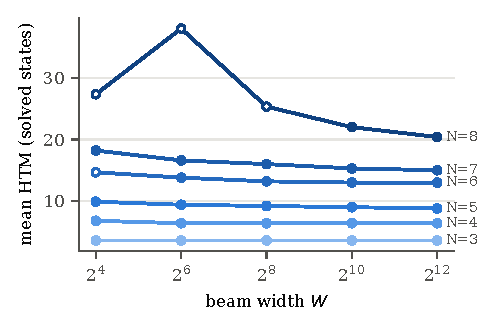
\includegraphics[width=\columnwidth]{figures/m4_width.pdf}
\caption{\Mfour: mean solution length against beam width $W$, one per-size network for each
Square size $N=3,\dots,8$ (10 states each; means over solved states). Hollow markers: not all 10
states solved, so the mean covers only the easier ones.}
\label{fig:m4width}
\end{figure}

\subsection{Does one network generalise across sizes?}
\label{sec:generalisation}

\begin{table}[t]
\caption{\FiveA, trained on Squares with $N\in\{4,\dots,8\}$ only: agreement of its distance
estimate with the true random-walk depth at the end of training, on fresh walks ($^\ast$ = size
never seen in training). RMSE is in units of $N^2/\ln N$.}
\label{tab:gen}
\small\setlength{\tabcolsep}{4pt}
\begin{tabular}{lrrrrrrrr}
\toprule
$N$ & 4 & 5 & 6 & 7 & 8 & 10$^\ast$ & 14$^\ast$ & 20$^\ast$ \\
\midrule
Pearson $r$ & 0.48 & 0.62 & 0.67 & 0.61 & 0.64 & 0.66 & 0.65 & 0.53 \\
normalised RMSE & 0.71 & 0.63 & 0.58 & 0.61 & 0.57 & 0.57 & 0.60 & 0.70 \\
\bottomrule
\end{tabular}

\end{table}

Table~\ref{tab:gen} shows that the distance estimate of \FiveA does not collapse on sizes it never
saw: its correlation with the true walk depth is \FiveACorrEight{} at $N=8$, the largest training
size, \FiveACorrTen{} at $N=10$ and \FiveACorrTwenty{} at $N=20$. These correlations are moderate;
a model of \FiveAParams{} parameters trained for \FiveASteps{} CPU steps is far from converged.

As a solver, \FiveA solved these fractions of instances: \FiveACoverage{}. With full-puzzle beam search it matched or came close
to \Mfour's per-size networks for $N\le6$, including the optimum on all ten \Sq{4} instances
(Table~\ref{tab:optimal}), but at $N=7$ six of ten full-puzzle searches used up their step limit
without reaching the goal: the search horizon, not time, was the problem. Inside
\FiveB's stages ($N\ge8$) it solved most states (the two \Sq{10} failures hit the 300\,s budget), with solutions shorter than \FiveB's own: on the
\PairedFiveAN{} instances both solved, \FiveB's solutions were \RatioFiveBFiveA$\times$ as long as
\FiveA's overall and \RatioFiveBFiveAUnseen$\times$ as long on the \PairedFiveAUnseenN{} instances
with $N>8$, sizes outside \FiveA's training range. The cost is time: transformer scoring on CPU
made \FiveA's staged solves several times slower than \FiveB's (Table~\ref{tab:square}). The one
\Sq{12} we tried did not finish within 900\,s, and we stopped the planned $N=12$ and $N=14$ runs
there; larger sizes need a GPU or a cheaper scoring path such as the move head.

\subsection{Ablations}
\label{sec:ablations}

\begin{table*}[t]
\caption{Ablations of \FiveB, removing one component at a time: macro actions, exact small stages,
the restriction of late center stages to pure-center commutators, the tables-only corner heuristic,
and the coarse abstraction tables (corners then use the MLP alone). Each cell: solved / tried, mean
HTM over solved states, mean seconds per state (failures included in time). Square: 5 states per size, 600\,s budget; cube: 2 states per
size, 300\,s budget. The same instances as Tables~\ref{tab:square} and \ref{tab:cube}.}
\label{tab:ablation}
\small
\begin{minipage}[t]{0.40\textwidth}\centering
\begin{tabular}[t]{@{}lrrrrrr@{}}
\toprule
Square & \multicolumn{3}{c}{$N=8$} & \multicolumn{3}{c}{$N=12$} \\
 & solved & HTM & s & solved & HTM & s \\
\midrule
full \FiveB & 5/5 & 59 & 0.9 & 5/5 & 144 & 4.5 \\
$-$ macros & 5/5 & 59 & 15 & 4/5 & 136 & 111 \\
$-$ exact stages & 5/5 & 67 & 0.5 & 5/5 & 175 & 4.0 \\
\bottomrule
\end{tabular}
\end{minipage}%
\hfill
\begin{minipage}[t]{0.56\textwidth}\centering
\begin{tabular}[t]{@{}lrrrrrr@{}}
\toprule
Cube & \multicolumn{3}{c}{$N=4$} & \multicolumn{3}{c}{$N=5$} \\
 & solved & HTM & s & solved & HTM & s \\
\midrule
full \FiveB & 2/2 & 246 & 31 & 2/2 & 452 & 74 \\
$-$ center restriction & 2/2 & 246 & 41 & 2/2 & 452 & 133 \\
corners: max(MLP, tab.) & 2/2 & 296 & 89 & 2/2 & 421 & 125 \\
$-$ coarse tables & 2/2 & 296 & 87 & 2/2 & 436 & 120 \\
\bottomrule
\end{tabular}
\end{minipage}%

\end{table*}

Table~\ref{tab:ablation} removes one component at a time.

\emph{Macro actions} are what make large Squares fast. Without them the \Sq{8} still solves at the
same length but takes \AblSquareNoMacrosNiTime\,s instead of \AblSquareFullNiTime\,s per state,
and at $N=12$ only \AblSquareNoMacrosNmSolved{} states solve within 600\,s
(\AblSquareNoMacrosNmTime\,s per state against \AblSquareFullNmTime\,s). A commutator turns a
``break, then restore'' detour, which the summed heuristic scores as uphill, into one downhill step.

\emph{Exact small stages} shorten solutions rather than speed them up: solving the frame optimally
instead of by beam search gives \AblSquareFullNiHTM{} instead of \AblSquareNoExactStagesNiHTM{} moves
at $N=8$ and \AblSquareFullNmHTM{} instead of \AblSquareNoExactStagesNmHTM{} at $N=12$.

On the cube, \emph{restricting late center stages to pure-center commutators} left lengths unchanged
here and saved time (\AblCubeFullNfTime\,s against \AblCubeNoCenterMacroRestrictionNfTime\,s per
\Cu{5} state). The \emph{corner heuristic} result is mixed: taking $\max(\text{MLP},\text{tables})$
instead of the tables alone made \Cu{4} solutions longer (\AblCubeCornerMlpPlusTablesNeHTM{}
against \AblCubeFullNeHTM{} moves) and \Cu{5} solutions shorter (\AblCubeCornerMlpPlusTablesNfHTM{}
against \AblCubeFullNfHTM{}), and was slower on both. Removing the coarse tables, so that corners fall back to the MLP alone,
gave the same pattern (\AblCubeNoCoarseTablesNeHTM{} and \AblCubeNoCoarseTablesNfHTM{} moves). With
two states per size we read these cube differences as indicative only; the clearest cube effect is
speed.

\subsection{Scaling with $N$ and lower bounds}
\label{sec:scaling}

\begin{figure*}[t]
\centering
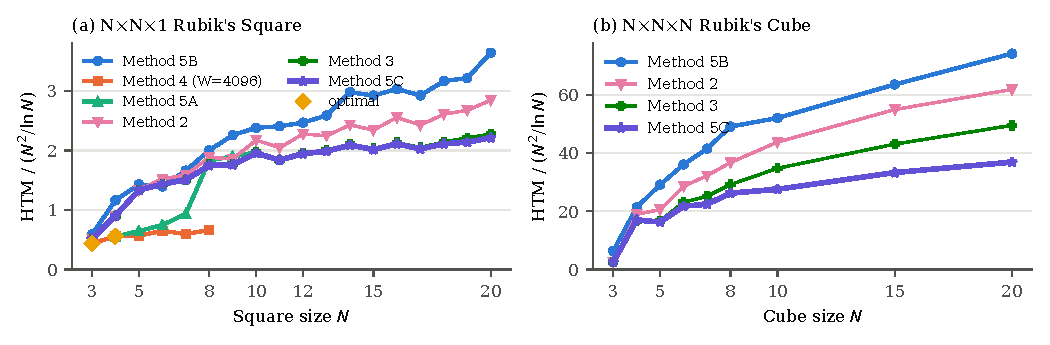
\includegraphics[width=\textwidth]{figures/scaling.pdf}
\caption{Solution length divided by $N^2/\ln N$, the growth rate of the worst case, for the Square
(a) and the cube (b). A flat line would mean growth at the rate of the worst case. Means over solved states;
the same instances as Tables~\ref{tab:square} and \ref{tab:cube}.}
\label{fig:scaling}
\end{figure*}

Figure~\ref{fig:scaling} divides each mean length by $N^2/\ln N$. For \FiveB on the Square this
ratio rises from \SqNormThree{} at $N=3$ to \SqNormTwenty{} at $N=20$, and on the cube it keeps
rising across the whole range. Over the sizes we can test, \FiveB's lengths therefore grow faster
than the $N^2/\log N$ rate that Demaine's construction achieves. The likely cause is that \FiveB
solves clusters a few at a time, while that construction amortises one move sequence over many
identical clusters. The per-size network of \Mfour sits well below
\FiveB where it exists.

\begin{table}[t]
\caption{Counting lower bounds on the worst case (God's number) in our move sets ($2N$ Square flips,
$9N$ cube half-turn moves), from the number of reachable center-cluster configurations as in
Demaine et al.~\cite{demaine2011algorithms}, next to \FiveB's mean length on random states. The
bounds are for the worst state, not for these instances.}
\label{tab:lb}
\small\setlength{\tabcolsep}{4pt}
\begin{tabular}{@{}rrrrr@{}}
\toprule
 & \multicolumn{2}{c}{Square} & \multicolumn{2}{c}{Cube} \\
\cmidrule(lr){2-3}\cmidrule(lr){4-5}
$N$ & lower bound & \FiveB mean & lower bound & \FiveB mean \\
\midrule
6 & 2 & 28 & 35 & 724 \\
8 & 5 & 62 & 75 & 1,510 \\
10 & 9 & 103 & 126 & 2,260 \\
15 & 18 & 243 & 262 & 5,280 \\
20 & 39 & 486 & 557 & 9,904 \\
\bottomrule

\end{tabular}
\end{table}

Table~\ref{tab:lb} puts the counting bounds next to our lengths. The bounds only say that
\emph{some} state needs that many moves, so they cannot certify optimality of any single solution,
but on the cube our lengths are more than an order of magnitude above them, so either the bounds
are very weak or there is much room left; both are likely.


%% =====================================================================
\section{Limitations}
\label{sec:limitations}

\begin{itemize}
\item \emph{Small samples and CPU only.} We test few states per size, especially for large cubes
  (one each at $N=15$ and $20$), so the large-$N$ comparisons rest on single instances; the gaps
  there are wide, but they are not tight estimates. Timings come from two different CPUs.
\item \emph{Still above Demaine's rate.} Every method's length divided by $N^2/\ln N$ still rises over
  the tested range, \FiveC's most slowly. We have not shown that any of them reaches the
  $\Theta(N^2/\log N)$ rate at these sizes.
\item \emph{\FiveC is greedy.} Its schedule looks at most one step ahead and treats which identical
  center sticker goes where as fixed; choosing those assignments so that clusters need the same next
  3-cycle, and a learned cost-to-go in place of the lookahead, are the obvious next steps. On the
  \Cu{4}, with one center and one wing cluster, there is nothing to batch and \FiveC is not shorter
  than \Mthree.
\item \emph{Exact search on the \Cu{3}.} With Korf's three databases on four cores, \Mone solves
  scrambles of 12 moves optimally but no random state within 30 minutes; larger pattern databases or
  a GPU would be needed for the standard benchmark.
\item \emph{\Mfour on cubes.} With 250$\times$ less training data than the original, our \Cu{3}
  model solved short scrambles but none of 10 random states at $W\in\{256, 1024, 4096\}$ and none of
  4 at $W=16{,}384$ (from the project's status log).
  This is a statement about our compute, not about the method.
\item \emph{\FiveA's evidence is preliminary.} One small Square model, a CPU budget, and no cube
  model.
\item \emph{Checker and sampling.} The checker enforces necessary conditions only, and random
  states come from long random walks rather than an exact uniform sampler.
\item \emph{Missing external baseline.} We did not run the dwalton76 NxNxN solver~\cite{walton2017nxnxn}
  on our instances.
\end{itemize}

%% =====================================================================
\section{Conclusion}

Decomposing Rubik's puzzles into clusters with $N$-invariant signatures lets one engine run seven
solvers on the same instances, from exact search to learned heuristics, for every size from 3 to 20.
Exact search settles the smallest Squares and shows how quickly it stops scaling; per-size networks
match the optimum where they exist; learned cluster-based search covers every size, and a
cluster-token network carries its distance estimates to sizes it never saw. At large $N$ the winner is
structural: Demaine's idea of fixing many clusters with one shared move sequence. Scheduling those
shared moves by net gain rather than by unanimous need, \FiveC solved the \Cu{20} in
\CuTwentyHTMFiveC{} moves, \FiveCGainTwenty\% fewer than Demaine's algorithm with 3-cycle batching
and \FiveCvsFiveBTwenty\% fewer than our staged beam search, with a lead that grows with $N$. Learning
that schedule is the natural next step, and the place where the two lines of this work meet. Code, data
and result files are available at \url{https://github.com/gauravrai1704/Rubik}.

\begin{acks}
This work was carried out as a course project at Shiv Nadar University.
\end{acks}

\bibliographystyle{ACM-Reference-Format}
\bibliography{references}

\end{document}
